%Gruppennummer
\newcommand{\Gruppe}{14}
\documentclass[12pt,a4paper]{article}

\usepackage[ngerman]{babel}
\usepackage[T1]{fontenc}
\usepackage[utf8]{inputenc}			% Umlaute

\usepackage{natbib}
\usepackage{url}
\usepackage{amsmath}
\usepackage{amssymb}
\usepackage{paralist}
\usepackage{geometry}
\usepackage{hyperref}
\usepackage{graphicx} 
\usepackage{float}
\usepackage{nicefrac} 
\usepackage{caption}
\usepackage{multicol}

\usepackage{amsfonts}
\usepackage{latexsym}
\usepackage{amssymb}
\usepackage{graphicx}
%\usepackage{picins}
\usepackage{amsmath}
\usepackage{amsthm}
\usepackage{array}
\usepackage{enumerate}
\usepackage{lastpage}

\usepackage{verbatim}
\usepackage{hyperref}

%\usepackage{lineno}		%	Zeigt Zeilennummern an
%\linenumbers					%	Aktivieren

\usepackage{url}		% Für urls
\usepackage{xspace}		% Korrekte Leerzeichen nach Makros
\usepackage{booktabs}

%\usepackage{mathabx}	% For convolution
\usepackage{rotating}	% For rotated graphics
\usepackage{fancyvrb}% Für R-Code (5.4.2009)



\renewcommand\arraystretch{1.3}
\newtheoremstyle{break}% name
{9pt}%      Space above, empty = `usual value'
{9pt}%      Space below
{}% Body font
{}%         Indent amount (empty = no indent, \parindent = para indent)
{\bfseries}% Thm head font
{}%        Punctuation after thm head
{\newline}% Space after thm head: \newline = linebreak
{}%         Thm head spec

\theoremstyle{break}
\newtheorem{auf}{Aufgabe}
\newtheorem{uebung}{Übungsaufgabe}

\geometry{a4paper, 
	top=25mm,
	left=20mm, 
	right=20mm, 
	bottom=25mm,
	headsep=7mm, 
	footskip=12mm}
\usepackage{fancyhdr}
\setlength{\parindent}{0em}
\pagestyle{fancy}
\fancyhf{}
\lhead{Data Mining 1}
\rhead{Gruppe \Gruppe}
\rfoot{\thepage}
\renewcommand{\headrulewidth}{1pt}
\renewcommand{\footrulewidth}{1pt}

\newcommand{\gqq}[1]{\glqq #1\grqq}    

\def\signed #1{{\leavevmode\unskip\nobreak\hfil\penalty50\hskip2em
		\hbox{}\nobreak\hfil(#1)%
		\parfillskip=0pt \finalhyphendemerits=0 \endgraf}}

\newsavebox\mybox
\newenvironment{aquote}[1]
{\savebox\mybox{#1}\begin{quote}}
	{\signed{\usebox\mybox}\end{quote}}

\setlength{\parskip}{0mm}
\setlength{\parindent}{0mm}


\stepcounter{secnumdepth}

\clubpenalty=4500		%	Vermeidet Schusterjungen
\widowpenalty=10000	% Vermeidet Hurenkinder


\newtheorem{hs}{Hilfssatz}
\newtheorem{examp}{Example}
\newtheorem{definition}{Definition}
\newtheorem{thm}{Theorem}
\newtheorem{prop}{Proposition}
\newtheorem{coro}{Corollary}
\newtheorem{lemma}{Lemma}
\newtheorem{conclusion}{Conclusion}
\newtheoremstyle{break}% name
{9pt}%      Space above, empty = `usual value'
{9pt}%      Space below
{}% Body font
{}%         Indent amount (empty = no indent, \parindent = para indent)
{\bfseries}% Thm head font
{}%        Punctuation after thm head
{\newline}% Space after thm head: \newline = linebreak
{}%         Thm head spec


%-------------------------------------------------------
%				Grafik-Verzeichnisse
%-------------------------------------------------------


%\graphicspath{{../..//}}

% 	Das Graphikverzeichnis befindet sich auf derselben Hierarchiestufe wie das Verzeichnis, das das Latex-Haupt-
% 	Dokument enthält!
% 	Die zwei // bewirken, dass alle Unterverzeichnisse durchsucht werden

%-------------------------------------------------------
%				Makros: Software, Euro
%-------------------------------------------------------
\newcommand{\Rsoft}{{\sffamily{R}}\xspace}
\newcommand{\Excel}{{\sffamily{Excel}}\xspace}
\newcommand{\myeuro}{\text{\euro}\xspace}
\newcommand{\EndBspl}{\hfill $\blacksquare$}
\newcommand{\myprozent}{\,\%\xspace}

%-------------------------------------------------------
%				Makros: Mathematik
%-------------------------------------------------------

\DeclareMathOperator{\e}{\mathrm{e}\xspace} %Euler e
\newcommand{\infimum}{\inf}
\newcommand{\nat}{{\mathbb N}}
\newcommand{\ganze}{{\mathbb Z}}
\newcommand{\reell}{{\mathbb R}}
\newcommand{\sumdots}{+ \ldots +}
\newcommand{\proddots}{\cdot \ldots \cdot}
\newcommand{\varorder}{\prec_{\textnormal{var}}}
\newcommand{\argmin}{\textnormal{argmin}}
%-------------------------------------------------------
%				Makros: Momente
%-------------------------------------------------------

\newcommand{\erw}{\textnormal{E}}
\newcommand{\var}{\textnormal{Var}}
\newcommand{\sd}{\textnormal{SD}}
\newcommand{\cov}{\textnormal{Cov}}
\newcommand{\cor}{\textnormal{Corr}}
\newcommand{\cv}{\textnormal{CV}}





%-------------------------------------------------------
%				Makros: Verteilungen
%-------------------------------------------------------

\newcommand{\Prob}{P} 

\newcommand{\NormVert}{\textbf{{N}}}
\newcommand{\BinVert}{\textbf{{Bin}}}
\newcommand{\NegBinVert}{\textbf{{NB}}} %Negative Binomialverteilung
\newcommand{\PoisVert}{\textbf{{Pois}}}
\newcommand{\ExpVert}{\textbf{{Exp}}}
\newcommand{\CompPoisVert}{\textbf{{CPois}}}
\newcommand{\ParetoVert}{\textbf{{Pareto}}}
\newcommand{\NullParetoVert}{\textbf{{Null-Pareto}}}
\newcommand{\GenPar}{\textbf{{GPD}}}    %Verallgemeinerte Pareto-Verteilung
\newcommand{\GleichVert}{\textbf{{U}}}
\newcommand{\GammaVert}{\Gamma}
\newcommand{\WeibullVert}{\textbf{{W}}}
\newcommand{\LogNormVert}{\textbf{{LN}}}
\newcommand{\LogGammaVert}{\textbf{{LN}}\Gamma}
\newcommand{\InvGaussVert}{\textbf{{IG}}}
%\newcommand{\BetaVert}{\beta}
\newcommand{\BetaVert}{\textbf{{Beta}}}
\newcommand{\PanjerVert}{\textbf{{Panjer}}}
%		Verteilungen
\newcommand{\GaussCop}{C^{\normalfont{Ga}}}
\newcommand{\GaussCopDichte}{c^{\normalfont{Ga}}}



%-------------------------------------------------------
%				Makros: Statistik
%-------------------------------------------------------
\newcommand{\MinP}{\textnormal{Min}\,$P$\xspace}

\newcommand{\err}{\textnormal{err}}
\newcommand{\bias}{\textnormal{Bias}}
%\newcommand{\variance}{\textnormal{variance}}
\newcommand{\mse}{\textnormal{MSE}}
\newcommand{\auc}{\textnormal{AUC}}
\newcommand{\logit}{{\textnormal{logit}}}
\newcommand{\betadach}{\widehat{\beta}}
\newcommand{\deltadach}{\widehat{\delta}}
\newcommand{\lambdadach}{\widehat{\lambda}}
\newcommand{\pidach}{\widehat{\pi}}
\newcommand{\pitilde}{\widetilde{\pi}}
\newcommand{\Gdach}{\widehat{G}}
\newcommand{\FDR}{\textnormal{FDR}}
\newcommand{\FDP}{\textnormal{FDP}}
\newcommand{\FWER}{\textnormal{FWER}}
\newcommand{\Bdach}{\widehat{B}}
\newcommand{\Cdach}{\widehat{C}}

%-------------------------------------------------------
%				Makros: Abkürzungen
%-------------------------------------------------------
\newcommand{\zB}{\mbox{z.\,B.}\xspace}
\newcommand{\xdh}{\mbox{d.\,h.}\xspace}
\newcommand{\bzgl}{\mbox{bzgl.}\xspace}
\newcommand{\vgl}{\mbox{vgl.}\xspace}
\newcommand{\Vgl}{\mbox{Vgl.}\xspace}
%\newcommand{\idr}{\mbox{i.\,d.\,R.}\xspace}
\newcommand{\idr}{{in der Regel}\xspace}
\newcommand{\evtl}{\mbox{evtl.}\xspace}
\newcommand{\Evtl}{\mbox{Evtl.}\xspace}
\newcommand{\etc}{\mbox{etc.}\xspace}
\newcommand{\usw}{\mbox{usw.}\xspace}
\newcommand{\bzw}{\mbox{bzw.}\xspace}
\newcommand{\oae}{\mbox{o.\,Ä.}\xspace}
\newcommand{\og}{\mbox{o.\,g.}\xspace}
\newcommand{\pa}{\mbox{p.\,a.}\xspace}
\newcommand{\uae}{\mbox{u.\,Ä.}\xspace}
\newcommand{\su}{\mbox{s.\,u.}\xspace}
\newcommand{\so}{\mbox{s.\,o.}\xspace}
\newcommand{\sog}{\mbox{sog.}\xspace}
\newcommand{\ua}{\mbox{u.\,a.}\xspace}
\newcommand{\uA}{\mbox{u.\,a.}\xspace}
\newcommand{\uU}{\mbox{u.\,U.}\xspace}
\newcommand{\uvam}{\mbox{u.\,v.\,a.\,m.}\xspace}
\newcommand{\ggf}{\mbox{ggf.}\xspace} % Neu: 3.6.2009
%	\newcommand{\iA}{\mbox{i.\,A.}\xspace}  Alte Version
\newcommand{\iA}{\mbox{i.\,Allg.}\xspace} %Neue Version 6.4.2009
\newcommand{\iW}{\mbox{im Wesentlichen}\xspace}
\newcommand{\xslash}{\,/\,} 		% 	Verwendung: blabal{\xslash}blabla
\newcommand{\entspricht}{\mathrel{\widehat{=}}}
%-------------------------------------------------------
%				Silbentrennung einzelner Ausdrücke
%-------------------------------------------------------


\begin{document}
	% Header
	\pagenumbering{roman}
\hspace{-1.4cm}
\parbox[b][80pt][b]{80pt}{
	
\includegraphics[width=200pt,height=100pt]{Bilder/hda_fbmn.png}}
\hfill
\parbox[b][75pt][t]{260pt}{
	\hspace*{\fill}\textbf{Gruppe \Gruppe} \\ 
	\hspace*{\fill} Carl Friedrich Gauß (161803) \\
	\hspace*{\fill} Hypatia von Alexandria (314159)\\
	\hspace*{\fill} Leonhard Euler (271828)}
\vspace{-0.2cm}
\hrule
\vspace{5mm}
\begin{center}
	{\bf\huge Data Mining 1\\[10mm]}
	{\bf \large Booklet von Gruppe \Gruppe}
\end{center}
\vspace{1cm}
\tableofcontents
\pagebreak
\addtocounter{secnumdepth}{-1}

	
	% Regelungen
	% \section*{Regelungen}
	\addcontentsline{toc}{section}{Regelungen}
	Für das Booklet in der Lehrveranstaltung \textit{Data Mining 1} gelten folgende Regelungen:
	\begin{itemize}
		\item Mindestens auf der Titelseite sollte der Gruppenname und die Namen aller Personen (incl. Maktrikelnummer) aufgeführt werden
		\item Einseitige Zusammenfassung (Executive Summary) mit den wichtigsten Ergebnissen am Anfang des Booklets
		\item Zu Beginn ein Inhaltsverzeichnis
		\item Ein Literaturverzeichnis nach dem Anhang
		\item Maximal 12 Seiten Inhalt (Mindestens Schriftgröße 11)
		\item Als Inhalt wird mindestens erwartet:
		\begin{itemize}[$\Rightarrow$]
			\item Beschreibung der Vorgehensweise bei den einzelnen Aufgaben (Algorithmus, Parameterwahl, etc.), Bewertung möglicher Alternativen
			\item Übersichtliche Darstellung der quantitativen Ergebnisse
			\item Interpretation der Ergebnisse bzgl. Aussagekraft, Anwendbarkeit der Methode, etc.
		\end{itemize}
		\item Code im Anhang
		\item Erstellung des Booklets mit \LaTeX
		\item Abgabe als PDF
	\end{itemize}
 % Auskommentieren!

	\pagebreak	
	\pagebreak
\section*{Zusammenfassung}
\addcontentsline{toc}{section}{Zusammenfassung}
	
	% Beginn Inhalt
	\pagebreak
	\pagenumbering{arabic}
	\section{Aufgabe 1: Entscheidungsbäume}
\subsection{Feature Engineering}

\subsubsection{Analyse der Zielvariable}
Wie Abbildung \ref{fig:disc_target_variable} entnommen werden kann, ist die Ausprägung der Zielvariable ungleich auf beide Klassen verteilt. Die Klassifizierungsgenauigkeit eines Modells muss demnach unter Berücksichtigung der sogenannten \emph{Null Accuracy} bewertet werden. Unter \emph{Null Accuracy} versteht man die Genauigkeit eines Modells, dass unabhängig von allen Eingaben immer die am häufigsten auftretende Klasse vorhersagt. In unserem Fall würde ein Modell, welches immer Regen vorhersagt, eine Klassifizierungsgenauigkeit von 79,39\% erreichen. Das Ziel der nachfolgenden Schritte ist also ein Modell mit einer besseren Klassifizierungsgenauigkeit als die \emph{Null Accuracy} aufzubauen.
\begin{figure}[ht]
	\centering
	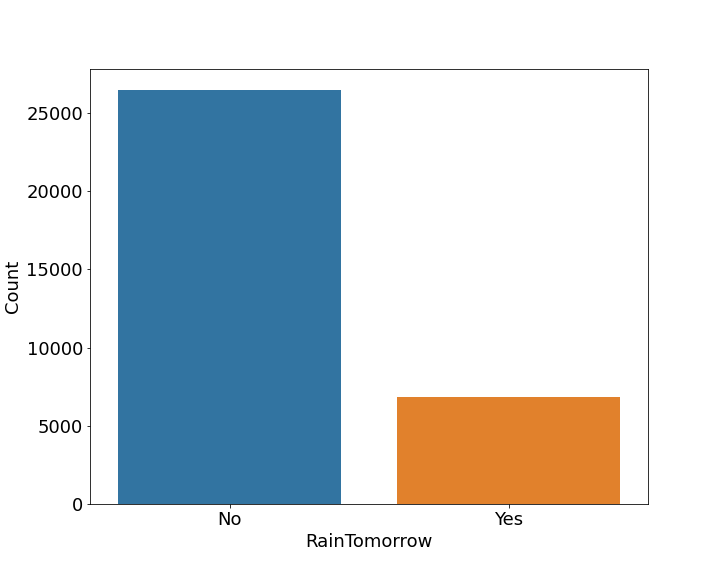
\includegraphics[width = 0.45\textwidth]{Bilder/distribution_target_variable.png}
	\caption{Verteilung der Zielvariable}
	\label{fig:disc_target_variable}
\end{figure}
\subsubsection{Fehlende Werte}
Der zu untersuchende Datensatz beinhaltet fehlende Werte. Im Folgenden werden Methoden beschrieben, wie mit den fehlenden Werte umgegangen wurde:
\begin{description}
	\item[Fehlende Zielvariable:]
	 Im ersten Schritt wurden alle Beobachtungen, welche keinen Wert für die Zielvariable \emph{RainTomorrow} aufweisen, aus dem Datensatz entfernt. Damit wurde die Anzahl an Beobachtungen um 834 auf 33402 reduziert.
	 \item[Spalten mit fehlenden Werten:]
	 In einem nächsten Schritt werden die Spalten aus dem Datensatz entfernt, in denen mehr als 40\% der beinhaltenden Variablen fehlen. Namentlich wurden somit die Spalten \emph{Evaporation, Sunshine, Cloud9am} sowie \emph{Cloud3pm} aus dem Datensatz entfernt. Der Schwellwert von 40\% wurde empirisch festgelegt und hat zu den besten Klassifizierungsergebnissen geführt.
	 \item[Beobachtungen mit fehlenden Werten]
	 Des Weiteren werden Beobachtungen aus dem Datensatz entfernt, von denen mehr als 50\% der Variablen fehlen. Durch diesem Schritt wurden 55 Beobachtungen aus dem Datensatz entfernt.
	 \item[Imputation]
	 Durch die zuvor beschriebenen Methoden ist der Datensatz immer noch  nicht frei von fehlenden Werten. Um diese zu ersetzen, werden für kategorische und numerische Variablen verschiedene Strategien zur Imputation verfolgt. Fehlende numerische Werte werden mit dem Median der jeweiligen Variable ersetzt. Der Median wurde gewählt, da dieser im Vergleich zum Mittelwert robuster gegenüber Ausreißern ist. Für kategorielle Variablen hingegen wird der am häufigsten vorkommende Wert verwendet. Wichtig bei der Ermittlung des Medians bzw. des häufigsten Wertes ist, dass dieser ausschließlich mit Hilfe der Trainingsdaten (siehe Abschnitt \ref{section:train_test_split}) ermittelt wird. Es muss davon ausgegangen werden, dass die Testdaten nicht bekannt sind. Die Ermittlung auf Basis des gesamten Datensatzes, inklusive der Testdaten, würde zu \emph{Data Leakage} führen und ist zu vermeiden. Die auf Basis der Trainingsdaten ermittelten Werte für die Imputation werden auf die Trainings- und Testdaten angewendet.
\end{description}

\subsubsection{Merkmalserstellung und Aufteilung}
Eine weit verbreitete Technik des Feature Engineerings ist die Erstellung zusätzlicher Merkmalen. Somit wurde die Variable \emph{MinMaxDiff} erstellt, welche die Differenz zwischen der minimalen und der maximalen Tages-Temperatur angibt. Des Weiteren wurden die Variablen \emph{PressureDiff, HumidityDiff und WindSpeedDiff} als Differenz der Beobachtungen am Morgen und Abend erstellt. Das Feld \emph{Datum} wurde in die Merkmale \emph{Year, Month} und \emph{Day} aufgeteilt.

\subsubsection{Diskretisierung}
%TODO: Entscheidungsbäume sind doch auch sensibel gegenüber vieler verschiedener Werte... Das wäre noch ein gutes Argument
Die Diskretisierung eines Merkmals kann eine Überanpassung bei der Erstellung von Modellen verhindern, indem der Wertebereich des Merkmals minimiert und somit generalisiert wird. Hierbei muss beachtet werden, dass der Informationsverlust durch die Diskretisierung nicht zu groß ist. Eine Diskretisierung wurde für das Merkmal \emph{Month} durchgeführt, indem es in das Merkmal \emph{Season} umgewandelt wurde. Das Merkmal \emph{Season} fasst immer 3 Monate zu einer Jahreszeit zusammen.

\subsubsection{Kodierung kategorischer Werte}
Um kategorische Werte für weitere Analysen verwenden zu können, müssen diese in numerische Werte umkodiert werden. Hierbei wurden die folgenden Strategien Angewendet:
\begin{description}
	\item[Binäre Kodierung]
	Die Zielvariable \emph{RainTomorrow}, sowie die Variable \emph{RainToday} liegen in den Ausprägungen \emph{Yes} und \emph{No} vor. Für eine weitere Verarbeitung wurden die Ausprägungen in eine numerische binäre Darstellung umgewandelt.
	\item[One-Hot-Kodierung]
	%TODO: One-Hot beschreiben?
	Das neu diskretisierte Merkmal \emph{Season} wird mittels \emph{One-Hot-Kodierung} umgewandelt. Eine \emph{Label-Kodierung}, also eine einfache Kodierung mit einem zufälligen Zahlenwert pro auftretender Variablenausprägung, hat den Nachteil, dass dadurch eine Variable entsteht, die gegebenenfalls metrisch interpretiert wird.
	\item[Ziel-Kodierung]
	Mit Hilfe der Ziel-Kodierung werden die Merkmale \emph{Location, WindGustDir, WindDir9am} und \emph{WindDir3pm} umgewandelt. Hierbei werden die Merkmalsausprägungen als ihren Einfluss auf die Zielvariable kodiert.
\end{description}

\subsubsection{Bereinigung von Ausreißern}
%TODO: Haben wirklich nur die Vairablen ausreißer?? Ich hatte nur die im code untersucht...
Ausreißer können die Performance eines Modells mindern, indem sie als Hebelwerte agieren und somit die Schätzungen der Zielvariable verzerren. Aus diesem Grund werden die Merkmale des Datensatz hinsichtlich ihrer Ausreißer begutachtet. Es wird ersichtlich, dass Merkmale wie \emph{Rainfall} und \emph{WindGustSpeed} abweichende Werte aufweisen. Das Entfernen dieser Werte aus dem Datensatz führt jedoch zu einer schlechteren Performance der im folgenden Abschnitt besprochenen Entscheidungsbäume. Deshalb werden die Beobachtungen nicht aus dem Datensatz entfernt.

\subsubsection{Normalisierung der Daten}
Für Entscheidungsbäume ist eine Normalisierung der Daten nicht Notwendig. Um das \emph{Feature Engineering} jedoch unabhängig vom gewählten Klassifizierer und auch im Hinblick auf neuronale Netze oder \emph{Support Vector Machines} (SVMs) durchzuführen, wird es an dieser Stelle durchgeführt. Die Werte der einzelnen Variablen werden dabei auf den Wertebereich $[0, 1]$ umskaliert.
 
\begin{comment}
\subsubsection{Variablenselektion}
%TODO: Brauchen wir die Variablenselektion wirklich? Oder wird das durch den Max_detph parameter vom Baum geregelt...?
Nach Abschluss der oben aufgeführten Schritte verfügt der Datensatz über 28 Einflussvariablen. Durch eine Variablenselektion soll die Anzahl dieser Einflussvariablen verringert werden. Das hat zum einen den Vorteil, dass Modelle  besser interpretierbar sind. Zum Anderen wird die Generalisierungsfähigkeit eines Modells erhöht, indem Merkmale ohne, oder nur mit geringem Einfluss auf die Zielvariable entfernt werden. Die Gefahr einer Überanpassung wird somit minimiert\\
\noindent \hspace*{7mm}
Für den betrachteten Datensatz wird eine univariate Variablenselektion mit dem Modul \emph{SelectKBest} der Bibliothek \emph{sklearn} durchgeführt. Dabei werden die \textit{k} Merkmale ausgewählt, die den höchsten Wert der F-Statistik aufweisen. Dieser Wert gibt an, ob ein einzelnes Merkmal einen signifikanten Einfluss auf die Zielvariable hat. $k$ wurde empirisch auf 5 festgelegt. Als Ergebnis wurden die Merkmale \emph{WindGustDir, Humidity9am, Humidity3pm, RainToday} und \emph{MinMaxDiff} ausgewählt.
%%%
\end{comment}


\vspace{1cm}
\subsection{Entscheidungsbäume}
\label{section:Entscheidungsbäume}
\subsubsection{Aufteilung in Trainings- und Testdaten}
\label{section:train_test_split}
Um das Modell nach Abschluss anhand der Klassifizierungsgenauigkeit bewerten zu können, sollte der Datensatz in Trainings- und Testdaten aufgeteilt werden. Die Aufteilung und eine anschließende Bewertung anhand der Testdaten ermöglicht eine Einschätzung der Generalisierungsfähigkeit des Modells. Als Aufteilungsverhältnis wurde 20\% Testdaten und 80\% Trainingsdaten gewählt. 20\% der Daten entsprechen 6670 Datensätzen und bilden eine ausreichend große Menge um die Modellgüte zu bestimmen. Die Wahl des Aufteilungsverhältnisses wurde außerdem nach den Empfehlungen aus \cite{geron2017hands-on} gewählt.

\subsubsection{Standard Einstellungen}
% Quelle: https://scikit-learn.org/stable/modules/generated/sklearn.tree.DecisionTreeClassifier.html\\
Der Entscheidungsbaum wurde mit Hilfe der \emph{scikit-learn}-Bibliothek erstellt \cite{scikit-learn}. Im ersten Aufgabenteil werden dazu die Standard-Einstellungen des Moduls genutzt. Diese sehen weder eine Beschränkung in der Tiefe des Baumes, noch Kriterien für eine Aufspaltung vor. Als Resultat wächst der Baum weiter, bis alle Blätter im Baum ausschließlich Werte einer Klasse enthalten. Das Ergebnis für die hier untersuchten Wetterdaten ist ein Baum, der sich an die Trainingsdaten überangepasst hat. In Abbildung \ref{fig:treedefault} ist ein Entscheidungsbaum mit den Standard-Einstellungen dargestellt. Die vielen Knoten und Blätter weisen auf eine Überanpassung an die Trainingsdaten hin. Ein weiterer Nachteil des Baums mit Standard-Einstellungen ist, dass die Entscheidungskriterien nur schwer interpretierbar sind. Ein weiterer Hinweis auf eine Überanpassung stellt die Korrektklassifizierungsrate der Trainingsdaten von 100\% dar. Zum Vergleich werden nur 79,18\% der Testdaten korrekt klassifiziert.


\subsubsection{Variationen}
Um einen leichter zu interpretierbaren und generalisierbaren Entscheidungsbaum erzeugen zu können, werden verschiedenen Einstellungen für die folgenden Hyperparameter angewandt. 


\begin{figure}[H]
    \centering
         \begin{minipage}{0.31\textwidth}
		\centering
		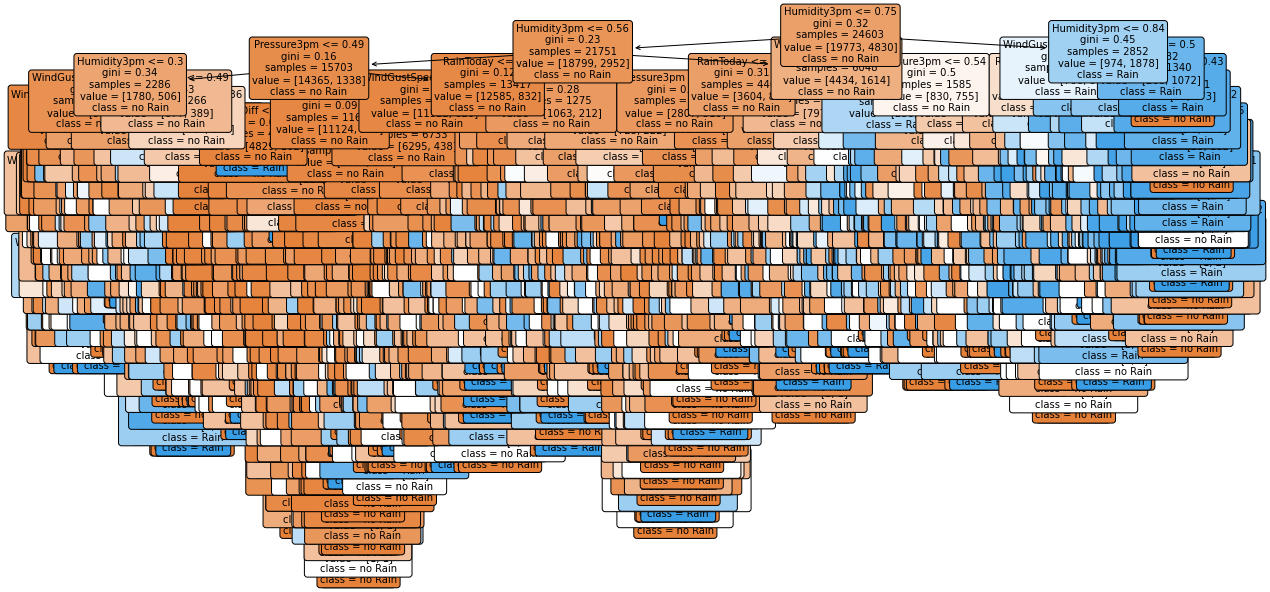
\includegraphics[width = 1\textwidth]{Bilder/treedefault}
		\caption{Entscheidungsbaum mit Default-Einstellungen}
		\label{fig:treedefault}
    \end{minipage}\hfill
     \begin{minipage}{0.31\textwidth}
        \centering
        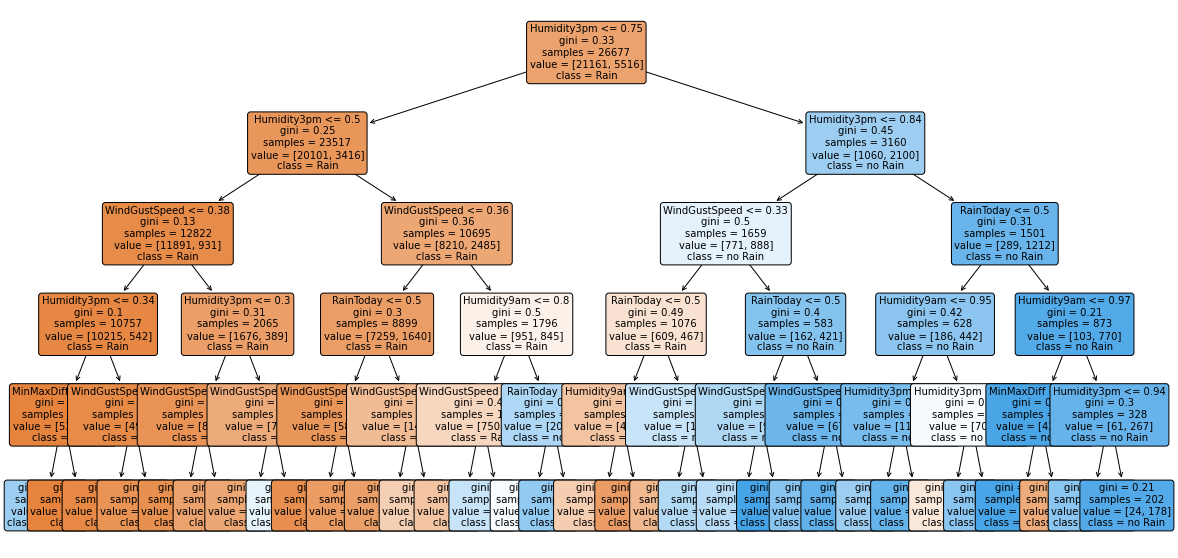
\includegraphics[width=1\textwidth]{Bilder/treeMaxDepth} % first figure itself
        \caption{Struktur eines Entscheidungsbaums mit \emph{max\_depth = 5}}
        \label{fig:treeMaxDepth}
    \end{minipage}\hfill
    \begin{minipage}{0.31\textwidth}
        \centering
        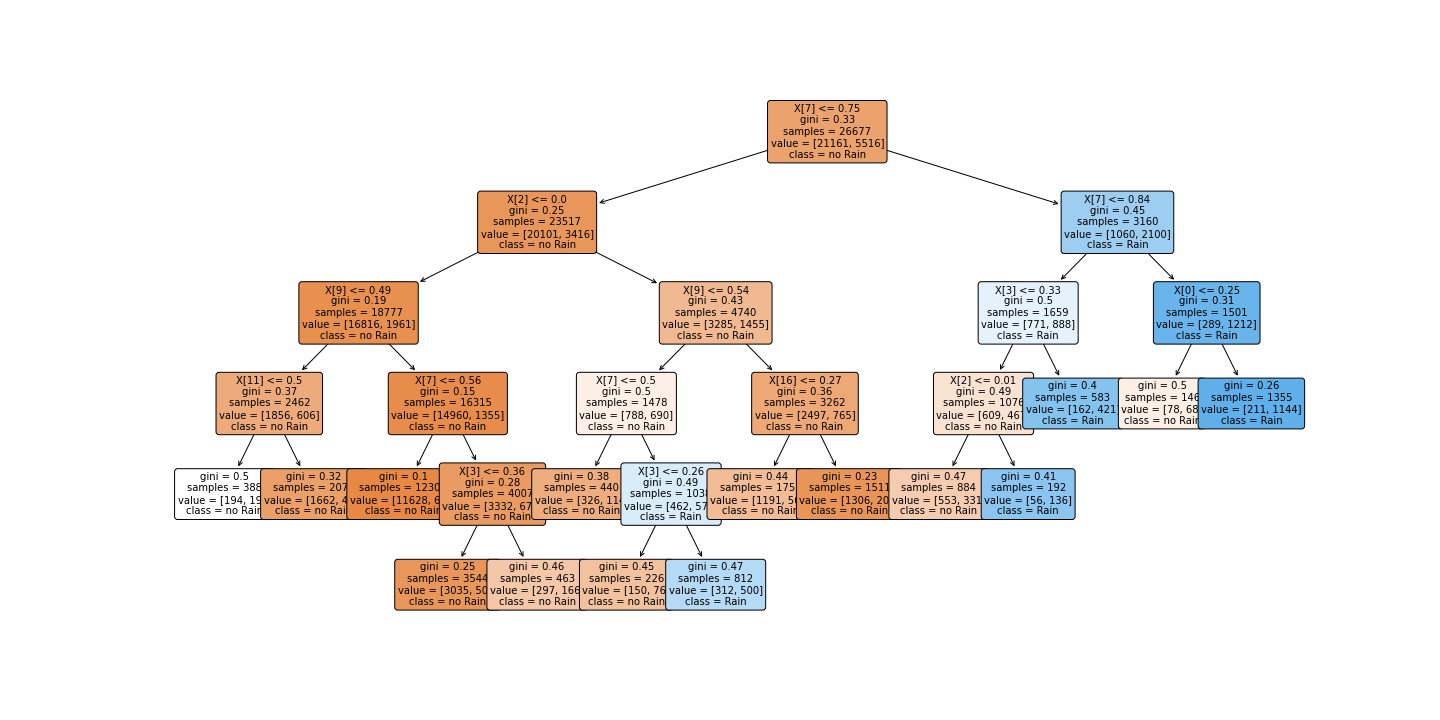
\includegraphics[width=1\textwidth]{Bilder/treeMinImpurityDecrease} % first figure itself
        \caption{Struktur eines Entscheidungsbaums mit \emph{min\_impurity\_decrease = 0.001}}
        \label{fig:treeMinImpurityDecrease}
    \end{minipage}\hfill
\end{figure}
\begin{comment}
Auf den Abbildungen \ref{fig:treeMaxDepth} bis \ref{fig:treeCriterion} sind exemplarisch Entscheidungsbäume dargestellt, deren Parameter empirisch festgelegt wurden. Bei der Visualisierung liegt der Fokus auf der Struktur des Baumes und nicht darauf, dass die einzelnen Knoten identifiziert werden können.\\
\end{comment}
\begin{description}
	\item[\emph{max\_depth}]
	 definiert die maximale Tiefe des Entscheidungsbaumes. Tiefe Bäume neigen dazu, sich den Trainingsdaten überanzupassen. Flache Bäume dagegen neigen dazu, die Trainingsdaten unteranzupassen. Auf Abbildung \ref{fig:grid_search_max_depth_tree} aus Kapitel \ref{section:univariat} ist die Balance zwischen über- und unteranpassung mit variierender \emph{max\_depth} dargestellt. Die beste Klassifizierungsgenauigkeit konnte mit einer maximalen Tiefe von 5 erreicht werden. Eine exemplarische Darstellung der Struktur eines Entscheidungsbaums der Tiefe 5 ist in Abbildung \ref{fig:treeMaxDepth} dargestellt.

	\item[\emph{min\_impurity\_decrease}] 
	legt fest, zu welchem Anteil die Unschärfe reduziert werden muss, sodass eine Aufteilung eines Knotens stattfindet. Dies hat, wie in Abbildung \ref{fig:treeMinImpurityDecrease} zu sehen, auch eine direkte Auswirkung auf die Tiefe des Entscheidungsbaums. Das Ergebnis einer \emph{Grid Search} nach einer optimalen Einstellung von \emph{min\_impurity\_decrease} kann Abbildung \ref{fig:grid_search_impurity_decrease} entnommen werden.
	
	\item[\emph{criterion}]
	definiert das Kriterium, an dem die Qualität einer Aufteilung gemessen wird. Die \emph{scikit-learn}-Bibliothek unterstützt hierbei den Gini-Index, und eine Messung des Informationsgewinns mittels der Entropie. Die Wahl des Gini-Index liefert hierbei unabhängig von den andern beiden Hyperparameter-Einstellungen ein minimal besseres Ergebnis. Außerdem ist die Berechnung des Informationsgewinns mit Hilfe der Entropie durch die logarithmische Funktion aufwändiger. In \cite{gini_entropy} wird der Unterschied zwischen Informationsgewinn und Gini-Index näher untersucht.
\end{description}

Wie bereits erwähnt haben die beiden Hyperparameter \emph{max\_depth} und \emph{min\_impurity\_decrease} eine Auswirkung auf die Tiefe des Entscheidungsbaums. Das Setzen von \emph{min\_impurity\_decrease} anstelle von  \emph{max\_depth} hat den Vorteil, dass dies eine eher weiche Abbruchbedingung während des Trainings darstellt. Somit ist die Gefahr der Unteranpassung geringer. Die Wahl des Gini-Index als Entscheidungskriterium für eine Aufteilung liefert minimal bessere Ergebnisse und ist unaufwändiger zu berechnen.


\begin{figure}[ht]
	\centering
	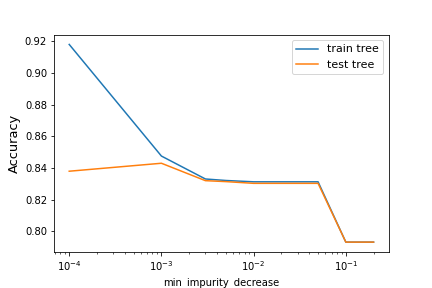
\includegraphics[width = 0.5\textwidth]{Bilder/min_impurity_decrease.png}
	\caption{Klassifizierungsgenauigkeit eines Entscheidungsbaums abhängig des Hyperparameters \emph{min\_impurity\_decrease}}
	\label{fig:grid_search_impurity_decrease}
\end{figure}

%TODO: Fazit und noch mal drüber lesen....

\subsubsection{Minimal Cost-Complexity-Pruning}
Eine Möglichkeit der Vermeidung des Overfittings bietet das \emph{Cost-Complexitiy Pruning} als sogenannte \emph{Post-Pruning}-Methode. Dabei wird der voll ausgebildete Baum iterativ beschnitten, indem diejenigen Teilbäume entfernt werden, die einen festgelegten penalisierten Fehlerterm minimieren.\\
\noindent \hspace*{7mm}
Das Modul \emph{DecisionTreeClassifier} bestimmt für jeden Knoten den effektiven $\alpha$-Wert. Dabei entpricht $\alpha_{eff}$ dem $\alpha$, für das gilt: $R_{\alpha}(T_{t})=R_{\alpha}(t)$. Der Knoten mit dem geringsten effektiven $\alpha$ wird vom Baum abgeschnitten. Dieses Vorgehen wird solange wiederholt, bis der geringste effektive $\alpha$-Wert größer als der gegebenen Penalisierungs-Term \emph{ccp\_alpha} ist.\\
\noindent \hspace*{7mm}
Dabei ist zu beachten, dass die Bäume stärker beschnitten werden, je höher der gegebene Penalisierungs-Term ist, da dieser eine hohe Anzahl an Knoten bestraft (siehe auch \ref{app:abb_booklet_1}).\\
\noindent \hspace*{7mm}
Das Pruning hat Auswirkungen auf die Modellgüte, indem es die Anpassung an die Trainingsdaten reguliert. Wird der Penalisierungs-Term zu hoch gesetzt, besteht die Gefahr der Unteranpassung, ein sehr niedriger Term führt zu Overfitting. In Abbildung \ref{fig:ccp_accuracyVsAlpha} ist beispielhaft für einen Entscheidungsbaum mit Default-Einstellungen die Trainings- und Testgenauigkeit (Accuracy) für verschiedene Pruning-Parameter $\alpha$ dargestellt.
\begin{figure}[h]
	\centering
	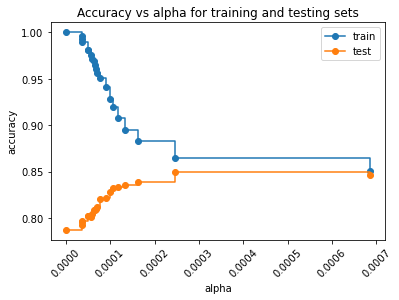
\includegraphics[width = 0.5\textwidth]{Bilder/ccp_accuracyVsAlpha.png}
	\caption{Trainings- und Testfehler für verschiedene $\alpha$-Werte}
	\label{fig:ccp_accuracyVsAlpha}
\end{figure}




	\pagebreak
\section{Aufgabe 2: Neuronale Netze}
\subsection{Neuronale Netze mit Numpy}
\subsubsection{Implementierung Backprop mit einem Hidden Layer}
\subsubsection{Hyperparameter}
Im folgenden werden Hyperparameter beschrieben, sowie ihre Auswirkungen auf das Neuronale Netzwerk diskutiert.
\begin{description}
	\item[Anzahl der Neuronen im Hidden Layer]\hfill \\
	%TODO: Eigentlcih sollte der Fehler auf die Trainingsdaten bei vielen Neuronen minimal sein. Irgendwie overfittet das Modell nicht klassisch.
	Wenn keine $l_1$ oder $l_2$ Regularisierung, Dropout \cite{dropout} oder andere Regularisierungstechniken eingesetzt werden, steigt die Gefahr einer Überanpassung mit steigender Anzahl an Neuronen im Netzwerk.   
	\begin{table}[ht]
		\centering
		\begin{tabular}{l|llllll}
			& 10000 & 1000 & 100  & 10   & 5    & 2    \\ \hline
			Test Fehler      & 62    & 19,9 & 14,9 & 14.9 & 14.9 & 15   \\
			Trainings Fehler & 188   & 43,5 & 35,1 & 35,0 & 35,0 & 35,1
		\end{tabular}
	\end{table}
	
	\item[Anzahl an Iterationen]\hfill \\
	Die Anzahl der Iterationen, die benötigt werden, bis der Trainingsfehler nicht mehr sinkt, hängt stark von der gewählten Lernrate ab. Im weiteren Verlauf wird das einmalige Iterieren durch den gesamten Trainingsdatensatz als Epoche bezeichnet. In Abbildung \ref*{fig:learning_rates} ist der Trainingsverlauf während mehrerer Epochen für verschiedene Lernraten abgebildet. Bei einer Lernrate von 0.1 sinkt der Trainingsfehler nach 100 Epochen nicht mehr.
	
	\item[Lernrate]\hfill \\
	%TODO: Bezug auf unser Beispiel herstellen
	Die Lernrate $\eta$ reguliert die Auswirkung eines einzelnen Schrittes im Gradientenabstiegsverfahrens. Eine hohes $\eta$ führt zu einer schnellen Minimierung des Trainingsfehlers. Jedoch steig die Gefahr, dass das Verfahren gute Minima überspringt, oder auch um ein gutes Minima Pendelt. Ein kleineres $\eta$ findet mit einer hohen Wahrscheinlichkeit ein besseres Minima, jedoch werden dafür mehr Iterationen benötigt \cite{neuronalenetze}.
	
	In Abbildung \ref*{fig:learning_rates} ist der Trainingsfehler während des Trainingsverlauf bei verschiedenen Lernraten dargestellt. Der Abbildung kann entnommen werden, dass für $\eta=0.01$ das Training nach 300 Epochen immer noch nicht konvergiert ist. Für $\eta=0.2$ ist zu sehen, dass das Verfahren sehr früh konvergiert und daher das Risiko besteht, dass wie oben beschrieben, gute Minima übersprungen wurden. Für komplexere Eingabedaten und Netzwerkarchitekturen würde dies ein reales Problem darstellen. In diesem einfachen Netzwerk und den einfachen Eingabedaten aus der Aufgabenstellung, kann auch mit $\eta=0.2$ ein gutes Ergebnis erreicht werden. Der Mittelweg beider Extreme bildet $\eta=0.1$ und wird als Einstellung vorgenommen.
	
	\begin{figure}[ht]
		\centering
		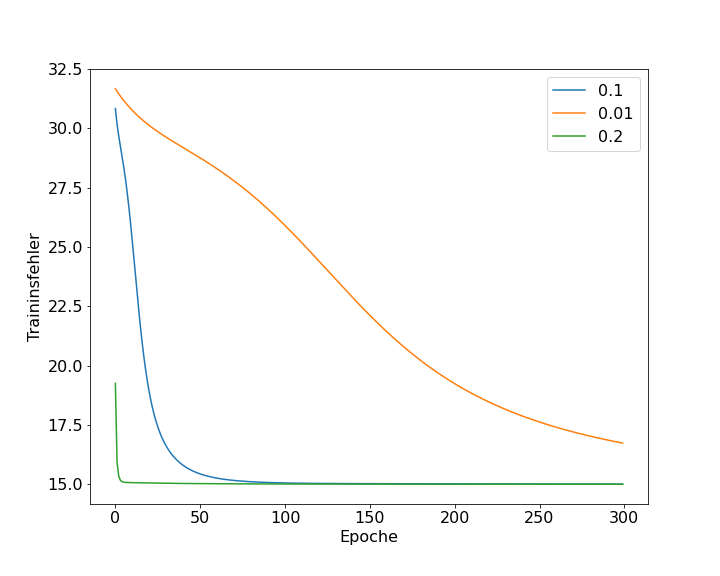
\includegraphics[width = 0.45\textwidth]{Bilder/learning_rates.png}
		\caption{Trainingsfehler während der Trainingsepochen bei verschiedenen Lernraten}
		\label{fig:learning_rates}
	\end{figure}
	
	\item[Initialisierung der Gewichte]\hfill \\
	Vor Allem beim Trainieren von tiefen neuronalen Netzen spielt die Initialisierung der Gewichte eine entscheidende Rolle um das Auftreten des Problems der explodierenden beziehungsweise verschwindenden Gradienten entgegen zu wirken \cite{geron2017hands-on}. In \cite{Glorot10understandingthe} wird die Glorot-Initialisierung, ein Verfahren zur Initialisierung der Gewichte bei Verwendung der Sigmoid Aktivierungsfunktion, beschrieben. Hierbei werden die Werte der initialen Gewichte aus einer Normalverteilung $\mathcal{N}(\mu,\,\sigma^{2})\,$ mit $\mu = 0$ und $\sigma^{2}=\frac{1}{fan_{avg}}$ entnommen. Hierbei gilt: 
	\[
	fan_{avg}=\frac{(fan_{in}+fan_{out})}{2}
	\]
	Wobei $fan_{in}$ der Anzahl an eingehenden Gewichte in einer Schicht entspricht und  $fan_{out}$ der Anzahl an Neuronen in der Schicht. Die Initialisierung der Gewichte in der vorliegenden Arbeit wurde  nach Glorot implementiert.

	%TODO: Muss noch mathematisch und schön. sollten die Schichten und Gewichte mathematisch anotieren. Die anotation dann unter Aufgabe 2.1
	Würden die Gewichte mit Null initialisiert werden, würde der Gradient für Alle Schichten bis auf die Ausgabeschicht Null sein. Ein Lernen würde nicht stattfinden. Der Gradient für die Aktualisierung der Gewichte zwischen versteckter Schicht und Ausgabeschicht würde für alle Partiellen Ableitungen gleich sein. Auch eine Initialisierung mit einer anderen Konstanten würde dazu führen, dass alle Gewichte "auf einer Ebene" gleich aktualisiert werden würden. Sie könnten einfach durch ein Neuron mit einer Verbindung ersetzt werden.
	
	Mithilfe der Verwendung eines \emph{Seeds} wird sicher gestellt, dass die zufällige Initialisierung der Gewichte bei jedem Durchlauf mit den gleichen Parametern die gleichen zufälligen Werte liefert. Das Netzwerk liefert also mit jedem Durchlauf bei gleichen Daten und Parametern die gleichen Ergebnisse. Somit wird die Reproduzierbarkeit im Netzwerk gefördert, was bei einer Fehlersuche und der Hyperparameter Optimierung hilfreich ist.
	
\end{description}
\subsection{Neuronale Netze mit TensorFlow}
%TODO: Beschreiben, welche Daten zum Trainieren genommen wurden
Im Folgenden wird die Implementierung eines voll vernetzen Neuronalen Netzwerks mit Hilfe der \emph{TensorFlow} Bibliothek beschrieben \cite{tensorflow2015-whitepaper}. Unterstützend wurde für den Aufbau des neuronalen Netzes die \emph{Keras}-API verwendet, die seit \emph{TensorFlow} Version 2 standardmäßig integriert ist. 

Um die Daten für das Training des Neuronalen Netzes effizient vorzubereiten wurde die \emph{Dataset}-API verwendet. Mit Hilfe der \emph{Dataset}-API wurde das zufällige Mischen der Trainingsdaten, sowie die Bereitstellung in Form von \emph{Mini-Batches} implementiert. Die Verwendung der \emph{Dataset}-API hat noch zusätzlich den Vorteil, dass die Ausführung von Vorbereitungsschritten der Daten perfekt mit dem Training des Neuronalen Netzes koordiniert und parallelisiert werden können.

\subsubsection{Normalisierung der Daten}
%TODO: Normalisierung der Daten beschreiben. Das ist für NNs Notwendig. Ohne Normalisierung kamen wir nur auf 79,8 % Genauigkeit.

\subsubsection{Hyperparameter Suche}
Um ein best Mögliches Modell für die vorliegenden Daten zu finden, wurde eine automatisierte Suche nach den besten Hyperparameter-Kombination implementiert. Die zur Auswahl stehenden Hyperparameter mit ihren möglichen Ausprägungen sind in Tabelle \ref{table:hyper} aufgeführt.

\begin{table}[ht]
	\centering
	\begin{tabular}{ll}
		\textbf{Hyperparameter}     & \textbf{Ausprägungen} \\ \hline
		Anzahl Hidden Layer         & 0,1,2,3,4             \\
		Anzahl Neuronen pro Schicht & 1,3,5,10,20,50,100    \\
		Lernrate                    & 0,1;  0,05;  0.01     \\
		Aktivierungsfunktion        & ReLU, Sigmoid, ELU \\
		Dropout Wahrscheinlichkeit  & 0;  0.25;  0.5       
	\end{tabular}
	\caption{\label{table:hyper}Learn rates during training the model.}
\end{table}

Durch begrenzte Ressourcen wäre eine Evaluierung aller möglichen Hyperparameter-Kombinationen mittels einer \emph{Grid Search} nicht möglich. In der vorliegenden Arbeit wurde deshalb eine zufällige Suche nach \cite{randomSearch} implementiert. Das Sieger-Modell aus 10 zufälligen Hyperparameter-Kombinationen htrainiat 4 versteckte Layer mit jeweils 3 Neuronen. Die Lernrate wurde auf 0.1 festgelegt und das Netzwerk wurde ohne die Verwendung von Dropout trainiert. Als effektivste Aktivierungsfunktion hat sich die ELU-Funktion herausgestellt \cite{elu}. Das Sieger-Modell konnte eine Klassifizierungsgenauikgkeit von 85,11\% auf die Testdaten erreichen. Die Daten zum trainieren und testen des neuronalen Netzwerks wurden analog zu Aufgabenstellung \ref{section:Entscheidungsbäume} verwendet.

	\section{Aufgabe 2: Ensemblemethoden}
\begin{table}[h]
	\begin{tabular}{|l|llll|}
		\hline
		& Entscheidungsbaum & AdaBoost & Random Forest & Bagging \\ \hline
		n\_estimators               &               &        100*          &   100    & \textbf{100}*    \\
		criterion                   &      gini         &            gini       &   gini       & entropy* \\
		max\_depth                  &    \textbf{5}*           &          \textbf{20}*          &    None      & 10*      \\
		min\_samples\_split         &     40*          &      2            &    \textbf{5}*      & 20*      \\
		min\_samples\_leaf          &     100*         &        1           &    1       & 10*      \\
		min\_weight\_fraction\_leaf &   0           &     0              &    0       & 0       \\
		max\_features               &         25*      &          None         &   5*       & 20*      \\
		max\_leaf\_nodes            &       None        &       None            &    None      & None     \\
		min\_impurity\_decrease     &     0          &       0            &    0      & 0     \\
		min\_impurity\_split        &        0.1*       &           0        &     0     & 0.1*     \\ \hline
	\end{tabular}
	\caption{\label{table:gridsearch} Optimale Hyperparameter-Einstellung pro Modell durch die univariate \emph{Grid Search}}
\end{table}

Im Folgenden Abschnitt wird die Implementierung und Optimierung verschiedener Ensemblemethoden und eines Entscheidungsbaums mit Hilfe der \emph{scikit-learn} Bibliothek beschrieben. Um einen Vergleich zwischen verschiedenen Ensemblemethoden herstellen zu können wurde das \emph{Bagging}- und \emph{AdaBoost}-Verfahren, sowie ein \emph{Random-Forest} implementiert. Alle drei \emph{Ensemblemethoden} wurden mit einem Klassifizierungsbaum als Basisklassifizierer erstellt. Die Klassifizierungsgenauigkeit der einzelnen Verfahren mit Standardeinstellungen, sowie nach einer Hyperparameter-Optimierung können in Tabelle \ref{table:results_grid} gefunden werden. 

\subsection{Hyperparameter Optimierung}
Um eine optimale Einstellung der Hyperparameter pro Verfahren zu finden, wurde mit Hilfe der \emph{scikit-learn} Bibliothek das \emph{Grid Search}-Verfahren implementiert. Im Gegensatz zu dem \emph{Random Search}-Verfahren, dass in Kapitel \ref{nn_hyperparams} verwendet wurde, sucht \emph{Grid Search} allen möglichen Hyperparameter-Kombinationen in einem gegebenen Parameterraum.  Als Metrik für die Optimierung wurde auf Grund der einfachen Interpretierbarkeit die Klassifizierungsgenauigkeit (engl. \emph{Accuracy}) gewählt.

\subsubsection{Univariat}
\label{section:univariat}
%TODO: Beschreibung wegen erweiterung des Parameterraums, falls das Optimum das maximum oder minimum des Raumes dargestellt hat.
Die aus der Aufgabenstellung angegebenen Hyperparameter wurden zunächst einzeln (univariat) variiert, um nach einem optimalen Wert pro Hyperparameter zu suchen. Pro Hyperparameter wird also ein einzelner Parameterraum definiert. Hierbei wurde die Suche in zwei Durchläufen durchgeführt. Der Hyperparameter, durch dessen Konfiguration weg von seiner Standardeinstellung, die größte positive Auswirkung auf die Klassifizierungsgenauigkeit erzielt werden konnte, wurde für den  nächsten Durchgang fest konfiguriert und aus dem zu suchenden Parameterraum entfernt. Die Ergebnisse der \emph{Grid Search} pro Modell und Hyperparameter sind in Tabelle \ref{table:gridsearch} dargestellt. Die \textbf{fett} geschriebenen Werte wurden jeweils nach dem Ersten der beiden \emph{Grid Search} Durchläufe festgelegt. Die Werte, die mit * gekennzeichnet sind, weichen von den Standardeinstellungen ab. Zu beachten ist, dass der Hyperparameter \emph{n\_estimators} durch eingeschränkte Rechenkapazitäten auf ein oberes Limit von 100 begrenzt wurde. Eine vollständige Auflistung der durchsuchten Parameterräume pro Hyperparameter ist in Tabelle \ref{table:parameter_grid_univariat} im Anhang zu finden.

In Abbildung \ref{fig:grid_search_max_depth_tree} ist  beispielhaft der erste Durchlauf einer \emph{Grid Search} nach dem Hyperparameter \emph{max\_depth} dargestellt. Es ist zu sehen, dass das \emph{Bagging}-Verfahren, sowie der \emph{Random Forest} robuster gegenüber einer Überanpassung an die Trainingsdaten sind. Zu beachten ist, dass die in der Abbildung dargestellten Kurven auf den Train- und Testdaten aus der 10-fachen Kreuzvalidierung basieren. 

%TODO: Testdaten bei cross validation.
\begin{figure}[ht]
	\centering
	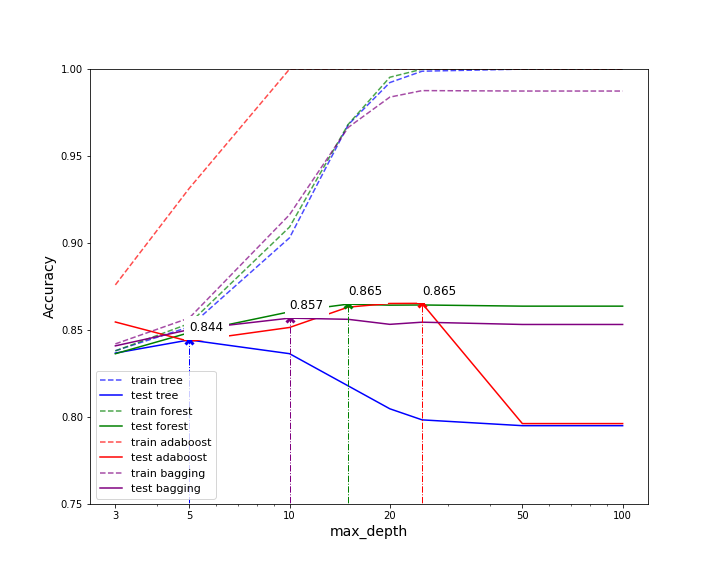
\includegraphics[width = 0.9\textwidth]{Bilder/grid_search_max_depth.png}
	\caption{Klassifizierungsgenauigkeit abhängig des Hyperparameters \emph{max\_depth}}
	\label{fig:grid_search_max_depth_tree}
\end{figure}

 
\subsubsection{Multivariat}
Im Gegensatz zu Abschnitt \ref{section:univariat} werden im folgenden Parameterräume definiert, die mehr als einen Hyperparameter umfassen. Somit können auch optimale Kombinationen von Hyperparameter-Einstellungen untersucht werden. Hierbei sollte darauf geachtet werden, dass die Rechenzeit einer \emph{Grid Search} exponentiell mit der Größe des Parameterraums ansteigt. Demnach werden folgende Hyperparameter von der Suche ausgeschlossen: \emph{n\_estimators}, \emph{min\_samples\_leaf}, \emph{criterion}, \emph{min\_weigh\_fraction\_leaf}, \emph{max\_leaf\_nodes} und \emph{min\_impurity\_split}. Die gewählten Parameterräume, sowie die gewählte Einstellung pro Hyperparameter ist in Tabellen \ref{table:parameter_grid_multivariat_forest} - \ref{table:parameter_grid_multivariat_bagging} im Anhang zu finden. Die Klassifizierungsergebnisse, der durch die multivariate \emph{Grid Serach} optimierten Verfahren, können in Tabelle \ref{table:results_grid} gefunden werden.

\subsubsection{Ergebnisse}
Die Klassifizierungsergebnisse der Verfahren mit Standard Einstellungen, sowie nach einer multivariaten und univariaten \emph{Grid Search} sind in Tabelle \ref{table:results_grid} zu finden. Wie der Tabelle entnommen werden kann, konnten die besten Klassifizierungsergebnisse mit der zweistufigen univariaten \emph{Grid Search} erzielt werden. Die Ergebnisse der Verfahren, die durch die multivariate \emph{Grid Search} optimiert wurden, können wahrscheinlich mit einer Erweiterung des Parameterraums verbessert werden. Dies würde jedoch auf der eingesetzten Hardware zu einem starken Anstieg der Berechnungsdauer führen. Als Alternative für weitergehende Untersuchungen könnte das in Abschnitt \ref{nn_hyperparams} eingesetzte \emph{Random Search} Verfahren angewendet werden.

\begin{table}[h]
	\begin{tabular}{lllll}
		\hline
		& Entscheidungsbaum & AdaBoost & Random Forest & Bagging \\ \hline
		Default Einstellungen         &    79.07\%               &  78,64\%        &  86,36\%             &  85,67\%       \\
		Nach zweistufiger\\
		univariater \emph{Grid Search}   &  84.77\%              &  86,64\%        &        86,43\%       &    86,13\%     \\
		Nach multivariater \emph{Grid Search} &  84,53\%                 &  86,64\%      &   86,34\%              &    85,97\%     \\ \hline
	\end{tabular}
	\caption{\label{table:results_grid} Klassifizierungsgenauigkeiten der Ensemblemethoden vor und nach der Optimierung durch \emph{Grid Search}}
\end{table}




	\pagebreak
\section{Aufgabe 4: Support Vector Machines}
\subsection{Unterkapitel 1}
\subsubsection{Unterkapitel 1.1}
	% Ende Inhalt
	
	% Anhang
	\pagebreak
	% \pagenumbering{Roman}
	\appendix
	\pagebreak
\pagenumbering{Roman}
\section{Anhang}
\subsection{Ergänzende Abbildungen zu Booklet Teil 1}
\label{app:abb_booklet_1}
Folgende Abbildungen stellen die Entscheidungsbäume der Cost-Complexity Aufgabe dar. Der Unterschied in den Bäumen mit geringerem und höherem $\alpha$ wird für die beiden Baum-Variationen gut ersichtlich. Abbildungen \ref{fig:ccp_fulltree_alpha_0005} und \ref{fig:ccp_fulltree_alpha_002} zeigen je einen vollständig ausgebildeten Baum, der durch Cost-Complexity \gqq{beschnitten} wurden.\\
\begin{figure}[H]
    \centering
     \begin{minipage}{0.45\textwidth}
        \centering
        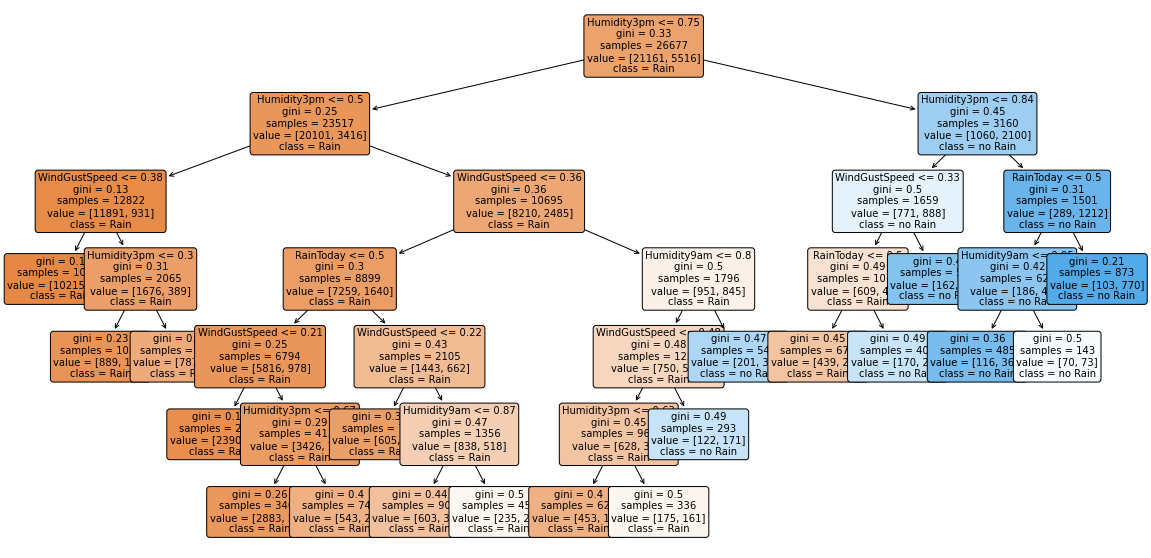
\includegraphics[width=0.9\textwidth]{Bilder/ccp_fulltree_alpha_0005.png}
        \caption{Entscheidungsbaum mit Parametern \emph{max\_depth=None} und \emph{ccp\_alpha=0.0005}}
        \label{fig:ccp_fulltree_alpha_0005}
    \end{minipage}\hfill
    \begin{minipage}{0.45\textwidth}
        \centering
        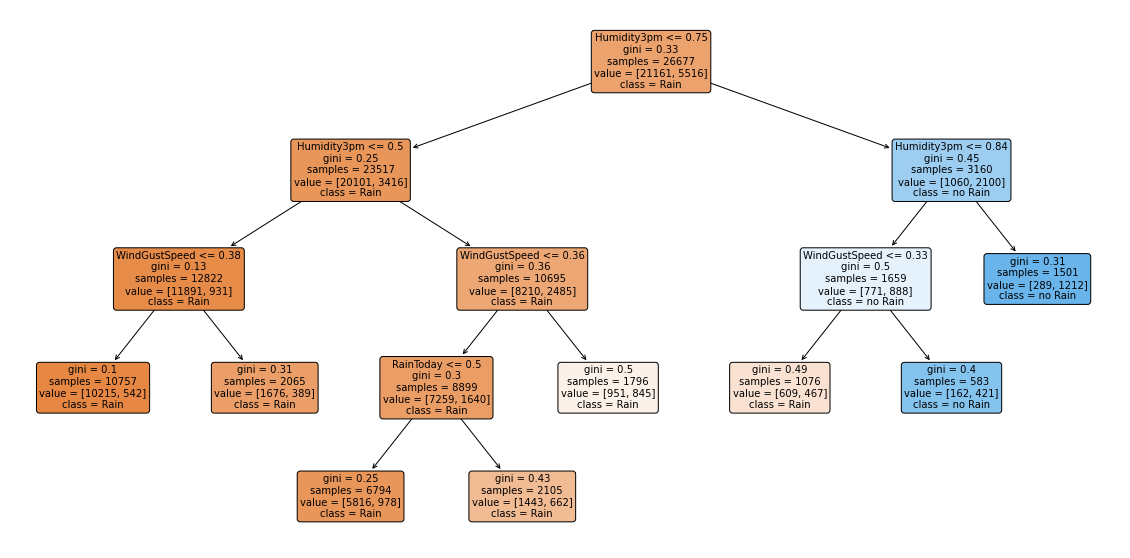
\includegraphics[width=0.9\textwidth]{Bilder/ccp_fulltree_alpha_002.png}
        \caption{Entscheidungsbaum mit Parametern \emph{max\_depth=None} und \emph{ccp\_alpha=0.002}}
        \label{fig:ccp_fulltree_alpha_002}
    \end{minipage}\hfill
\end{figure}
Abbildungen \ref{fig:ccp_maxDepth_alpha_001} und \ref{fig:ccp_maxDepth_alpha_004} zeigen je einen beschnittenen Baum der mit der Einstellung \emph{max\_depth = 8} erstellt wurde.
\begin{figure}[H]
    \centering
     \begin{minipage}{0.45\textwidth}
        \centering
        \includegraphics[width=0.9\textwidth]{Bilder/ccp_maxDepth_alpha_001.png}
        \caption{Entscheidungsbaum mit Parametern \emph{max\_depth=8} und \emph{ccp\_alpha=0.001}}
        \label{fig:ccp_maxDepth_alpha_001}
    \end{minipage}\hfill
    \begin{minipage}{0.45\textwidth}
        \centering
        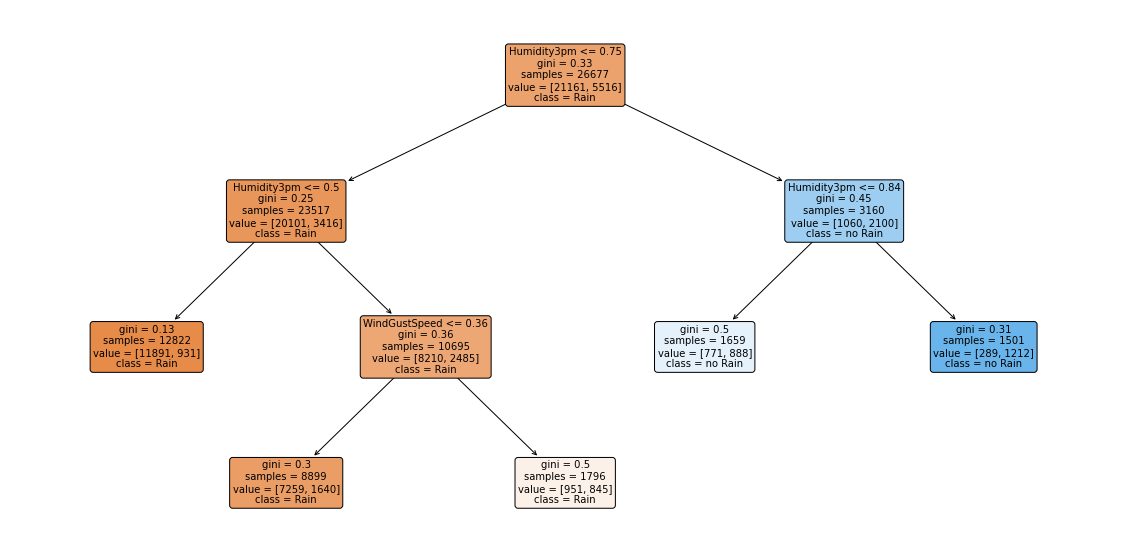
\includegraphics[width=0.9\textwidth]{Bilder/ccp_maxdepth_alpha_004.png}
        \caption{Entscheidungsbaum mit Parametern \emph{max\_depth=8} und \emph{ccp\_alpha=0.004}}
        \label{fig:ccp_maxDepth_alpha_004}
    \end{minipage}\hfill
\end{figure}
\pagebreak
\subsection{Quellcode zu Booklet Teil 1}
\pagebreak
\subsection{Ergänzungen zu Booklet Teil 2} \label{app:ergaenzung_booklet_2}
Folgend ist die mathematische Herleitung der Backpropagation für das in Aufgabe 1 gegebene Modell aufgeführt.\\\\
y: Beobachtete Werte der Stichprobe\\
$a_{2}=\hat{\pi}$\\
$\sigma$ = Sigmoid-Funktion
\begin{align*}
    dW_{2} &= \frac{\partial E^{n}}{\partial W_{2}}\\
    &= \frac{\partial E^{n}}{\partial z_{2}}\cdot \frac{\partial z_{2}}{\partial W_{2}}\\
    &= \frac{\partial E^{n}}{\partial a_{2}} \cdot \frac{\partial a_{2}}{\partial z_{2}} \cdot \frac{\partial z_{2}}{\partial W_{2}}\\
    &= \frac{\partial }{\partial a_{2}} \frac{1}{2}(y-a_{2})^{2} \cdot \frac{\partial }{\partial z_{2}} \sigma(a_{1}W_{2} + b_{2})\cdot \frac{\partial }{\partial W_{2}}(a_{1}W_{2}+b_{2})\\
    &= -(y-a_{2}) \cdot \sigma(a_{1}W_{2}+b_{2})(1-\sigma(a_{1}W_{2}+b_{2}))\cdot a_{1}\\
    &= \left[ -\begin{pmatrix}
        y_{1}  -  a_{2;11} \\
        \vdots \\
        y_{n}  -  a_{2;n1}  \\
        \end{pmatrix} \cdot \begin{pmatrix}
                            \sigma (z_{2;11}) \\
                            \vdots \\
                            \sigma (z_{2;n1})  \\
                            \end{pmatrix} \cdot \begin{pmatrix}
                                                    1-\sigma (z_{2;11}) \\
                                                    \vdots \\
                                                    1-\sigma (z_{2;n1})  \\
                                                    \end{pmatrix}\right]^{T} \cdot \begin{pmatrix}
                                                                        a_{1;11} & \cdots & a_{1;1m} \\
                                                                        \vdots & \ddots & \vdots \\
                                                                        a_{1;n1}&\cdots & a_{1;nm}  \\
                                                                        \end{pmatrix}\\\\
    \Rightarrow \delta_{2} &= \frac{\partial E^{n}}{\partial z_{2}}\\
     \delta_{2} &= -(y-a_{2}) \cdot \sigma(a_{1}W_{2}+b_{2})(1-\sigma(a_{1}W_{2}+b_{2}))\\\\
    db_{2} &= \frac{\partial E^{n}}{\partial b_{2}}\\
    &= \frac{\partial E^{n}}{\partial a_{2}} \cdot \frac{\partial a_{2}}{\partial z_{2}} \cdot \frac{\partial z_{2}}{\partial b_{2}}\\
    &= -(y-a_{2}) \cdot \sigma(a_{1}W_{2}+b_{2})(1-\sigma(a_{1}W_{2}+b_{2})) \cdot 1\\
    &=\left[-\begin{pmatrix}
        y_{1}  -  a_{2;11} \\
        \vdots \\
        y_{n}  -  a_{2;n1}  \\
        \end{pmatrix} \cdot \begin{pmatrix}
                            \sigma (z_{2;11}) \\
                            \vdots \\
                            \sigma (z_{2;n1})  \\
                            \end{pmatrix} \cdot \begin{pmatrix}
                                                    1-\sigma (z_{2;11}) \\
                                                    \vdots \\
                                                    1-\sigma (z_{2;n1})  \\
                                                    \end{pmatrix}\right]^{T} \cdot \begin{pmatrix}
                                                                            1 \\
                                                                            \vdots \\
                                                                            1  \\
                                                                            \end{pmatrix} \\\\
    dW_{1} &= \frac{\partial E^{n}}{\partial W_{1}}\\
    &= \delta_{1} \cdot X\\\\
\end{align*}
\begin{align*}    
    \Rightarrow \delta_{1} &= \frac{E^{n}}{\partial z_{1}}\\
    &= \sum_{k} \frac{\partial E^{n}}{\partial z_{2}}\cdot \frac{\partial z_{2}}{\partial z_{1}}\\
    &= \sum_{k} \delta_{2} \cdot \frac{\partial z_{2}}{\partial z_{1}}\\
    &= \sum_{k} \delta_{2}\cdot \frac{\partial }{\partial a_{1}}(a_{1}W_{2}+b_{2})\cdot \frac{\partial }{\partial z_{1}}\sigma(X\cdot W_{1} +b_{1})\\
    &= \sum_{k} \delta_{2}\cdot W_{2} \cdot \sigma(X\cdot W_{1}+b_{1})(1- \sigma(X\cdot W_{1}+b_{1}))\\
    \Rightarrow dW_{1}&= \delta_{2} \cdot \begin{pmatrix}
                        w_{2;11} \\
                        \vdots \\
                        w_{2;m1} \\
                        \end{pmatrix} \cdot \begin{pmatrix}
                                            \sigma (z_{1;11})& \cdots & \sigma(z_{1;1m}) \\
                                            \vdots & \ddots &\vdots\\
                                            \sigma (z_{1;n1}) & \cdots & \sigma (z_{1;nm})  \\
                                            \end{pmatrix} \cdot \begin{pmatrix}
                                                                1-\sigma (z_{2;11}) \\
                                                                \vdots \\
                                                                1-\sigma (z_{2;n1})  \\
                                                                \end{pmatrix} \cdot \begin{pmatrix}
                                                                                         x_{11} & x_{12}\\
                                                                                         \vdots & \vdots\\
                                                                                         x_{n1} & x_{n2}\\
                                                                                        \end{pmatrix} \\\\
    db_{1} &= \delta_{1} \cdot \frac{\partial}{\partial b_{1}}\sigma(X\cdot W_{1}+b_{1})\\
    &= \delta_{1} \cdot 1\\
    &= \delta_{2} \cdot \begin{pmatrix}
                        w_{2;11} \\
                        \vdots \\
                        w_{2;m1} \\
                        \end{pmatrix} \cdot \begin{pmatrix}
                                            \sigma (z_{1;11})& \cdots & \sigma(z_{1;1m}) \\
                                            \vdots & \ddots &\vdots\\
                                            \sigma (z_{1;n1}) & \cdots & \sigma (z_{1;nm})  \\
                                            \end{pmatrix} \cdot \begin{pmatrix}
                                                                1-\sigma (z_{2;11}) \\
                                                                \vdots \\
                                                                1-\sigma (z_{2;n1})  \\
                                                                \end{pmatrix} \cdot 1
\end{align*}
\subsection{Quellcode zu Booklet Teil 2} \label{app:quellcode_booklet_2}
\pagebreak
\subsection{Quellcode zu Booklet Teil 3}
\subsection{Ergänzende Tabellen zu Teil 3}

\begin{table}[h]
	\centering
	\begin{tabular}{ll}
		\hline
		Hyperparameter              & Parameterraum                              \\ \hline
		n\_estimators               & {[}10, 50, 100{]}                          \\
		criterion                   & {[}gini, entropy{]}                    \\
		max\_depth                  & {[}None, 3,5,10, 15, 20, 25, 50{]}         \\
		min\_samples\_split         & {[}2, 5,10, 20, 30, 40{]}                  \\
		min\_samples\_leaf          & {[}1, 2, 5, 10, 20, 40, 100, 200{]}                  \\
		min\_weight\_fraction\_leaf & {[}0, 0.2, 0.4, 0.5{]}                     \\
		max\_features               & {[}None, 5, 10, 15 ,20, 25{]}              \\
		max\_leaf\_nodes            & {[}None, 2 ,10, 100, 150, 200, 300, 500{]} \\
		min\_impurity\_decrease     & {[}0.0, 0.001, 0.002, 0.01, 0.1{]}     \\
		min\_impurity\_split        & {[}0.0, 0.1, 0.2, 0.5, 0.8, 1, 2, 3{]}     \\ \hline
	\end{tabular}
	\caption{\label{table:parameter_grid_univariat} Parameterräume der univariaten \emph{Grid Search}}
\end{table}

\begin{table}[h]
		\centering
\begin{tabular}{lll}
	\hline
	Hyperparameter          & Parameterraum                       & Gewählter Parameter \\ \hline
	max\_depth              & {[}None, 5, 10, 15{]}               & None                \\
	min\_samples\_split     & {[}2, 5, 10{]}                      & 5                   \\
	max\_features           & {[}None, 5, 20, 25{]}               & None                \\
	min\_impurity\_decrease & {[}0.00005, 0.0001, 0.001, 0.003{]} & 0.00005             \\ 
	n\_estimators &  & 100 \\ \hline
\end{tabular}
	\caption{\label{table:parameter_grid_multivariat_forest} Parameterräume und Ergebnisse der multivariaten \emph{Grid Search} des Random Forest}
\end{table}


\begin{table}[]
	\centering
	\begin{tabular}{lll}
	\hline
	Hyperparameter          & Parameterraum                       & Gewählter Parameter \\ \hline
	max\_depth              & {[}None, 5, 10, 15{]}               & None                \\
	min\_samples\_split     & {[}2, 5, 10{]}                      & 5                   \\
	max\_features           & {[}None, 5, 20, 25{]}               & None                \\
	min\_impurity\_decrease & {[}0.00005, 0.0001, 0.001, 0.003{]} & 0.00001             \\ \hline
\end{tabular}
	\caption{\label{table:parameter_grid_multivariat_tree} Parameterräume und Ergebnisse der multivariaten \emph{Grid Search} des Entscheidungsbaums}
\end{table}

\begin{table}[]
	\centering
	\begin{tabular}{lll}
	\hline
	Hyperparameter          & Parameterraum                        & Gewählter Parameter \\ \hline
	max\_depth              & {[}None, 5, 10, 20. 25{]}                & 20                   \\
	min\_samples\_split     & {[}2, 5, 10, 20{]}                   & 2                  \\
	max\_features           & {[}None, 5, 20, 25{]}                & None                  \\
	min\_impurity\_decrease & {[}0.0, 0.0001, 0.0005, 0.001{]} & 0.0             \\ 
	n\_estimators &  & 100 \\ \hline
\end{tabular}
	\caption{\label{table:parameter_grid_multivariat_adaboost} Parameterräume und Ergebnisse der multivariaten \emph{Grid Search} des Adaboost-Verfahrens}
\end{table}

\begin{table}[]
	\centering
	\begin{tabular}{lll}
	\hline
	Hyperparameter          & Parameterraum                        & Gewählter Parameter \\ \hline
	max\_depth              & {[}None, 5, 10, 15{]}                & None                \\
	min\_samples\_split     & {[}2, 5, 10, 20{]}                   & 10                  \\
	max\_features           & {[}None, 5, 20, 25{]}                & 5                   \\
	min\_impurity\_decrease & {[}0.00005, 0.0001, 0.0005, 0.001{]} & 0.0001              \\ 
	n\_estimators &  & 100 \\ \hline
\end{tabular}
	\caption{\label{table:parameter_grid_multivariat_bagging} Parameterräume und Ergebnisse der multivariaten \emph{Grid Search} des Bagging-Verfahrens}
\end{table}



\pagebreak
\subsection{Quellcode zu Booklet Teil 4}
	
	\pagebreak
	\addcontentsline{toc}{section}{Literatur}
	\bibliography{lit}
	\bibliographystyle{chicago}
\end{document}

